%In his Inaugural Lecture at University College London, Dr. Peter B. Medawar defined for the fist time \textsl{ageing} as merely surviving the years, ignoring the increased deterioration and decay. 
%He proposed at the same time to use the word \textsl{senescence} for those processes, stating that it should mean decline of vitality \cite{Medawar1952}.
%Interestingly, he made these definitions in his lecture \quotes{An Unsolved Problem in Biology}, also remarking how much things had changed in 50 years in terms of mortality.
%Dr. Medawar noticed how the principal causes of death shifted from infective towards cancer and cardiovascular diseases, both with a certain genetic susceptibility.
%And so, a basis for considering ageing as subjected to the forces of Natural Selection was established.
%Not many years later, in 1958, Theodosius Dobzhansky defined ageing as the decline of homoeostasis, linking it again to the affairs of natural selection.
%This definition is much closer to the one we work with currently, whereby ageing is the decay of biological fitness, which in itself refers to an evolutionary term.

In 1958, Theodosius Dobzhansky published an essay discussing the relation between homoeostasis and senility, and how natural selection affects both \cite{Dobzhansky1958}.
On it, Dobzhansky reflected on the concept of homoeostasis, defined by Walter Cannon some years before as the \quotes{wisdom of the body} \cite{Cannon1934}, or the ability to, through controlled changes in the organism, adapt to changes in the eviroment, provided that they are within the \quotes{normal} changes the organism had evolved to withstand.
He also linked this concept with ageing, by defining the later as the reduction of this adaptability or plasticity agains \quotes{normal} enviromental changes.
Specifically, he proposed that \quotes{\textsl{the homeostatic buffering against enviromental shocks is weakened during the postreproductive phase}}.

In his work \quotes{The Causes of Evolution}, Haldane considered this topic without any clear conclusion.
To him, natural selection \quotes{may either favor or hinder the prolongation of life during the postreproductive phase} \cite{Haldane1933}.
To Dobzhansky, the fact that homoeostatic mechanisms \quotes{tend to deteriorate during the autumm of life}, while the same function most efficiently during youth and maturity, is indication of how these are fashioned by natural selection.
Of course, we now understand in much more detail how far the link between homoeostasis and ageing goes, knowing specific cell paths, cellular systems, and other homoeostasis mechanisms for which \emph{heritable} malfuction (or even slightly under-optimal function) is a cause for a hastened ageing process.

After decades of tentative work on these determinants of ageing, in 2013, a seminal work finally established a precise framework to study how genetic determinants and their interaction with the environment regulates this process \cite{Lopez-Otin2013}. 
The framework is based on nine \emph{hallmarks of ageing}.

\section{Hallmarks of ageing} \label{s_intro_hallmarks}

Ageing is quasi-universal among multicellular organisms, yet, it is probably one of the least-understood of the natural processes of our biology \cite{Kirkwood2005}.
It can be described as a progressive loss of biological fitness, or the progressive decline in functional integrity and homoeostasis, culminating in death \cite{Singh2019}.
As such, it is expected to be caused by a continuous accumulation of damage with points of inflexion, at which the attempts of the body of fighting this creeping decay adds to the deleterious nature of ageing.

The characterization of the hallmarks of ageing, much like what happened with the hallmarks of cancer previously published \cite{Hanahan2011}, has helped conceptualize the underlying nature of ageing whilst setting a frame in its study.

For its categorization, each hallmark must satisfy 3 key principles:

\begin{enumerate}[topsep=1ex,itemsep=-1ex]
    \item It should manifest under normal ageing.
    \item Its experimental aggravation should accelerate the normal ageing process.
    \item Its experimental betterment should delay the normal ageing process, increasing healthspan and lifespan.
\end{enumerate}

Following this canon, nine hallmarks were defined.
These were genomic instability, telomere attrition, epigenetic alterations, loss of proteostasis, deregulated nutrient sensing, mitochondrial dysfunction, cellular senescence, stem cell exhaustion, and altered intercellular communication.
These nine hallmarks were grouped in 3 categories, depending on their impact on the process of ageing.
The first category, \emph{primary hallmarks}, is composed of those considered to be the causes of cellular damage, including genomic instability, telomere attrition, epigenetic alterations, and loss of proteostasis.
The second category, (\emph{antagonistic hallmarks}), was defined as the group of compensatory or antagonistic responses to the damage produced by the primary hallmarks.
While these responses are able to initially mitigate the damaging effects produced by the primary hallmarks, after becoming chronic they will turn deleterious as well.
This group includes deregulated nutrient sensing, mitochondrial dysfunction, and cellular senescence.
Lastly, \emph{integrative hallmarks}, which arise from the consequences of the previous groups, are directly responsible for the functional decline associated with ageing.
This category consists of two hallmarks, stem cell exhaustion, and altered intercellular communications \cite{Lopez-Otin2013}.

\begin{figure}[t!]
    \begin{center}
        \includegraphics[width=\textwidth]{figures/hallmarks.pdf}
        \caption[The hallmarks of ageing]{\footnotesize The nine hallmarks of ageing, grouped by category using the different colours.
        In \textcolor{myred1}{\textbf{red}} are displayed the primary hallmarks, such as genomic instability, telomere attrition, epigenetic alterations, and loss of proteostasis.
        In \textcolor{myora1}{\textbf{orange}} we can see the secondary or antagonistic hallmarks, \textit{i.e.} deregulated nutrient sensing, mitochondrial dysfunction, and cellular senescence.
        Finally, those in \textcolor{myaqu1}{\textbf{green}} are the integrative hallmarks, namely, stem exhaustion, and altered intercellular communication.}
        \label{f_hallmarks}
    \end{center}
\end{figure}

\subsection{Primary hallmarks} \label{ss_intro_hallmarks_primary}

\emph{Genomic instability} refers to the gradual accumulation of genetic damage throughout life \cite{Moskalev2013}.
As we age, the integrity and stability of our DNA\nomenclature{DNA}{Deoxyribonucleic Acid} is being continuously challenged by both exogenous and endogenous threats.
Physical, chemical and biological agents such as  ultraviolet light, mutagenic substances, or even viral replication are some examples of exogenous damage that DNA must withstand.
In addition, DNA faces internal sources of instability, such as replication errors, or the damage produce by some by-products of our own metabolism, like ROS\nomenclature{ROS}{Reactive Oxygen Species} \cite{Hoeijmakers2009}.
Overall, the genome is constantly suffering highly diverse lesions, including point mutations, translocations, chromosomal gains and losses, telomere shortening, and gene disruption caused by the integration of viruses and transposons.
For that reason, organisms have evolved a complex network of DNA repair mechanisms capable of tackling most of this problems \cite{Lord2012}.
Excessive DNA damage, or insufficient DNA repair favours the ageing process.
On the other hand, incorrect handling of this repair process is in itself one of the sources of further damage to the DNA.
Thus, many lesions are originated after mismatch repair, non-homologous end-joining, translesion synthesis, or base excision repair \cite{Agathangelou2018}.
Hence, these aquired complex systems and characteristics are subject to heredity and hence to the forces of natural selection, adding weight to the hypothesis of heritable longevity \cite{Lord2012}.

The aforementioned damage to the DNA is seemingly random in location, but there are some specific chromosome regions that are specially susceptible to age-related dam\-age, such as the telomeres.
Telomeres, a genomic region made up of repeated sequences at the end of each chromosomal arm, are among such regions, making \emph{telomere attrition} another primary hallmark.
This reduction in length that accompanies ageing originates from the natural incapability of the DNA polymerase to completely replicate the terminal ends of linear DNA molecules \cite{Turner2019}.
There is a specific DNA polymerase capable of replicating this \quotes{caps}, known as telomerase, but it is not expressed by most of mammalian cell types, leading to the progressive reduction of this DNA segment over time \cite{Shay2016}.
Researchers have observed not only a natural reduction of telomere size during normal ageing, but also that the pathological dysfunction of telomerase in experimental models greatly accelerates the process of ageing.

As we advance in the field of epigenetics, we increasingly recognise the importance of its physiological and pathological role in a lot of different biological processes, including ageing.
For this reason, we include \emph{epigenomic alterations} as one of the primary hallmarks of ageing.
These modifications affect all cells and tissues throughout life, via DNA methylation, post-translational modification of histones, and chromatin remodelling, and can be linked to accelerated ageing processes \cite{Pal2016}.
For instance, it has been experimentally observed that specific epigenetic alterations can mimic progeroid syndromes in model organisms\cite{Osorio2010}.
%Furthermore, enhancing the epigenetical function of SIRT6 has shown to increase the healthy lifespan, while decreasing it seems to diminish longevity \cite{Kanfi2012}.
Because of this, understanding and manipulating the epigenome holds promise for improving age-related pathologies, hence extending lifespan and, more importantly, healthspan.

The last primary hallmark of ageing, \emph{loss of proteostasis}, relates to the maintenance of a correct protein homoeostasis in the cell, meaning, getting rid of defective proteins, or correcting them.
The function of most proteins depends on their tridimensional structure, hence a misfolded protein could either not have function at all or have a different, unregulated one.
Specifically, we use the term \quotes{proteostasis} to reffer collectively to all the paths that deal with unfolded or misfolded proteins, namely the autophagy path, proteasome and lysosome degradation paths, and refolding via chaperones \cite{Klaips2018}.
These paths can be regulated based on the action of the heat-shock protein family \cite{Hartl2011,Koga2011,Mizushima2008}.
%Whenever these paths suffer alterations, unfolded or misfolded proteins remain in the cell and tend to aggregate, generating pathologies and hastening ageing.
In a normal situation, the different pathways works coordinatedly towards restoring the structure of misfolded peptides or to remove and degrade them completely, avoiding the accumulation of damaged (and damaging) proteins \cite{Powers2009}.
Numerous studies have shown that ageing tends to alter proteostasis, decreasing its effectiveness \cite{Hipp2019}.
When this happens, it has been observed that chronic accumulation of misfolded proteins may lead to age-related pathologies, such as Alzheimer and Parkinson's disease, or cataracts \cite{Powers2009}.
Finally, when inducing perturbations in this system, age-associated pathologies as well as hastened ageing has been observed.
In contrast, by improving proteostasis we can achieve the opposite effect and delay ageing \cite{Zhang2008}.

\subsection{Antagonistic hallmarks} \label{ss_intro_hallmarks_secondary}

The \emph{deregulation of nutrient sensing} hallmark relates to the system that detects and corrects the levels of different nutrients, energy, and other elements that alter body homoeostasis.
This complex hallmark stems from the relationship between anabolic signalling and accelerated ageing \cite{Fontana2010}.
As an example of this, a pharmacological manipulation that mimics low availability of nutrients has been observed to extend longevity in mice \cite{Harrison2009}.
Also, consistent with this, dietary restriction has shown to increase healthy lifespan in several species, including some primates \cite{Mattison2017}.
% Demasiado escueto? Es un tema un poco complejo para entrar a saco pero igual podemos mencionar algo de la glucosa? O será meterse en un maizal?

Ageing also affects the respiratory chain, whose efficacy diminishes with age, increasing electron leakage and reducing ATP\nomenclature{ATP}{Adenosine TriPhosphate} generation \cite{Green2011}.
We know this hallmark as \emph{mitochondrial dysfunction}.
In turn, these problems tend to increase the concentration of ROS, which, as mentioned before, also plays an important role in accelerating ageing \cite{Harman1965}.
While this association between defects in the respiratory chain and hastened ageing has being known for a long time, major details remain a research challenge.
In fact, the fulfilment of the third principle of hallmarks (amelioration leading to higher lifespan) is still under discussion.

\emph{Cellular senescence} is defined as a stable arrest of the cell cycle coupled with phenotypic changes \cite{Campisi2007,Kuilman2010}.
Several ageing-related stimuli are believed to trigger this process, including telomere shortening, non-telomeric DNA damage, and depression of the INK4/ARF locus \cite{Collado2007}.
The accumulation of senescence cells in a tissue can be indirectly measured through surrogate markers, such as DNA damage or the presence of metabolites such as senescence-associated $\beta$-galactosidase \cite{Dimri1995}.
It has been observed that these senescent cells are not equally accumulated across tissues in old age.
In fact, some organs, like heart or kidney, do not show changes in senescence associated to age \cite{Hoenicke2012,Kang2011,Xue2007}.
It has been widely assumed that senescent cells contribute to ageing, however, cellular senescence should be considered a response from the body to ageing, by marking cells for their deletion.
Sadly, as we age, due to all the other problems associated, the mechanisms that should get rid of these \quotes{marked} cells function suboptimally, and the deletion does not happen as fast as it should (or at all) \cite{Calcinotto2019}.
Therefore, it is the process of ageing which promotes the accumulation of senescent cells that otherwise should have been killed and removed.
Thus, the malfunction of the turnover system that replaces cells in tissues lowers the regenerative capacity of the progenitor cells and leads to their exhaustion.

\subsection{Integrative hallmarks} \label{ss_intro_hallmarks_integrative} %actualizar referencias

As we previously stated, these hallmarks are the direct result of the previous ones.
Its chronification is the final cause for most of the phenotypic changes associated with ageing.
And so, as a direct response to cellular senescence, the first of these hallamarks is \emph{stem cell exhaustion}.
It can be defined as the decline in the regenerative potential of tissues.
For instance, it has been shown that haematopoietic stem cells of aged mice decrease in cell-cycle activity compared to those of young mice \cite{DeHaan2018,Shaw2010}.
Of course, this directly correlates with a higher accumulation of DNA damage and over-expression of cell-cycle arrest proteins such as p16\textsuperscript{INK4a} \cite{Janzen2006,Rossi2007,Stenvinkel2017}.
While a deficit in proliferation is detrimental for the long-term maintenance of the organism, its excess is equally damaging, since it translates into an early exhaustion of the proliferating capacity of the stem cells of the tissue.
This effect has been observed in experiments with \textit{Drosophila melanogaster} intestinal stem cells, where excessive proliferation lead to exhaustion and premature ageing \cite{Rera2011,Wang2014}.
As an integrative hallmark, stem-cell exhaustion can be modulated by interventions on primary and antagonistic hallmarks.
For instance, it has been shown that inducing \textit{INK4a} (related to cellular senescence), or decreasing IGF-1 (related to deregulated nutrient sensing), we can help preserve the quiescence of stem cells, delaying stem cell exhaustion in the organism \cite{Chakkalakal2012,Tumpel2019}.

Besides cell-autonomous alterations, ageing also involves changes at the level of cell-cell integration, either by endocrine, neuronal or neuroendocrine paths \cite{Laplante2012,Rando2012,Zhang2013}.
Thus, \emph{altered intercellular communication}, the last hallmark of ageing, has ubiquitous effects in several different signalling paths, including a deregulation in neurohormonal signalling (such as renin-angiotensin, adrenergic or insulin-IGF1 signalling) \cite{Bocheva2019}.
This provokes an increase in inflammatory reactions, a decrease in immunosurveillance against both pathogens and premalignant cells, and also changes in the composition of the peri- and extracellular environment.
One of the most interesting effects of an altered intercellular communication is a smouldering proinflammatory phenotype associated with ageing called \emph{inflammageing} \cite{Franceschi2014}.
Inflammaging has different causes, such as an accumulation of proinflammatory tissue damage, a failure of an immune system to effectively clear pathogens or dysfunctional cells, propensity to secrete proinflammatory cytokines by senescent cells, or an autophagic response \cite{Franceschi2017,Salminen2012}.
% Lo mismo que en derregulation of nutrient sensing... Dado que es uno de los que luego tienen mas importancia en cachalote y tortuga, debería explayarme algo más?

%\subsection{Ageing as a progressive loss of function decline} \label{ss_intro_hallmarks_ageing}
%
%Having stabilised the main routes affected by longevity, I'd like to further discuss how this process takes place, by progressively increasing the difficulty in maintaining the homoeostasis. [Something on those lines, \cite{Kirkwood2005} may be useful].

\section{The Degradome}

As clearly reflected by the hallmarks of ageing, ageing is an extremely complex trait, with multiple intertwined systems, and a network of causes and consequences that extend to almost any remarkable cellular pathway.
A useful step in tackling these complexities is to separate a simpler system that nevertheless recapitulates some of the characteristics of the whole system.
In this regard, we have extensively worked on \emph{proteases}, \textit{i. e.}, proteins capable of degrading other proteins by means of peptide bond hydrolysis in an essentially irreversible way \cite{Perez-Silva2015}.
Proteases influence diverse biological features of the organisms, such as the immune system, digestion process, skin regeneration, cell cycle progression, tissue remodelling, neuronal outgrowth, haemostasis, wound healing, angiogenesis, apoptosis or metastasis, \cite{Lopez-Otin2008,Quiros2015,Reinhard2015,Voskoboinik2015}.

Due to these ubiquitous functions, the proper function of the proteolytic system is key to maintain homoeostasis in the organism, so it must be tightly regulated in terms of both activation and specificity.
Failings in their regulation underlie very diverse pathological conditions, such as progeria, cancer or even mental illness\cite{Turk2012}.
Thus, this set of genes experienced a remarkable evolutive expansion as an adaptation to regulate the large set of substrates depending on its correct functioning.

The large number of protease genes \cite{Perez-Silva2015} and their interdependence led to the definition of the \emph{degradome} as the complete set of proteases in a given organism \cite{Lopez-Otin2002a}.
The set of techniques that study and characterise proteases in this context is known as \emph{degradomics}. 
Given the large amount of information we often work with when delving in degradomics, bioinformatic techniques are important tools, as they allow researchers to focus on the biological meaning of the data and not its processing. 
Our experience and the mining of literature are usually a vital complement to the manual curation of annotations after automatic predictions and other analysis.
All together aimed towards finding links between protease alterations and pathological consequences, including hereditary diseases, sometimes referred as \emph{degradomopathies} \cite{Quesada2009}

\section{Molecular strategies against ageing and model organisms} \label{s_intro_models}

With information on hallmarks of ageing and the influence of proteases on them, we can look for clues on how longevity affects the genome of long lived animals.
The abundant data on protease function and biochemistry can then be leveraged to discern some of the molecular mechanisms that underlie extended life-span.
As controls, we can use evolutionary comparison with both close and distant relatives of diverse longevity.

\subsection{\textit{Physeter macrocephalus} and other Cetacea} \label{ss_intro_models_sperm_whale}

The sperm whale is a marine mammal, part of the Cetacea infraorder.
As such, they are part of the order Artiodactyla\footnote{Sometimes referred as Cetartiodactyla, a combination of \quotes{Cetacean} and \quotes{Artiodactylia}, arguing that despite the clear evidence supporting this clade, the enormous morphological differences between cetaceans and the rest justify this distinction.} (also known as even-toed ungulates), placing them as relatives to Camelidae (suborder Tylopoda), the pig and close family (suborder Suina), the ruminants (suborder Ruminantia), and hippopotamuses (with whom Cetacea share the Whippomorpha suborder; figure \ref{f_cetacean_tree}) \cite{Agnarsson2008}.
Cetacea and Sirenia (the order of manatees or sea cows) are the only mammals that live their entire lives inside the water.
Interestingly, they are not closely related to those, nor to Superfamily Pinnipedia (seals and the like), the only other mammal adapted to semiaquatic life \cite{Arnason2007,Tabuce2008}.
This suggests that aquatic adaptation developed independently several times in Mammalia, an example of convergent evolution.
On its own, Cetacea is further divided into two parvorders, Odontoceti, to which the sperm whale belongs, and Mysticeti \cite{Mancia2018}.

\textsl{Mysticeti} or \quotes{Baleen Whales} feed on plankton, by using a filter-like system based on extremely thin keratin bristle-like structures called baleen (as in its \quotes{common} name \cite{Fordyce2018}.
The fifteen members composing this parvorder are quite diverse, ranging in size from the 6 $m$ and 3,000 $kg$ of the pygmy right whale to the 31 $m$ and 190,000 $kg$ of the blue whale \cite{Agnarsson2008,Wada2003}.
They also diverge in other features, such as life expectancy and diving capacity.
Of special interest in the present work is the Bowhead whale (\emph{B. mysticetus}), some of whose specimens have been shown to live over 400 years, the largest life span recorded among Mammalia \cite{Keane2015}.
In addition, the availability of genomic data on Minke whale (\emph{B. acutorostrata}) allows genetic comparisons, as both whales are representatives of the Mysticeti parvorder \cite{Yim2014c}.

\textsl{Odontoceti} or toothed whales, are those presenting teeth.
These cetaceans feed on meat from various species, from aquatic mammals to fishes, including, in the case of the sperm whale, giant squids \cite{Best1979}.
As found in the parvorder of the Mysticeti, there is great divergence between members of this group as well, with species ranging from 1.5 $m$ and 50 $kg$ to more than 20 $m$ and 50,000 $kg$ \cite{Warren2017a}.
Odontoceti is a much larger parvorder than Mysticeti, with more than 70 different species \cite{Agnarsson2008}.
As a reflection of this diversity, Odontoceti are further divided in \textsl{Physeteroidea}, the superfamily comprising the sperm whales and relatives; \textsl{Delphinoidea}, including all salt-water dolphins and relatives (\textit{e.g.}, the killer whale, or the \textsl{Monodontidae} family, composed of narwhals and beluga whales); \textsl{Ziphioidea}, the superfamily of the beaked whales (\textit{e.g.}, Cuvier's whale); and 3 other superfamilies that include the fresh-water dolphins, \textsl{Inioidea}, \textsl{Platanistoidea}, and \textsl{Lipotoidea} (figure \ref{f_testudines_tree}) \cite{Agnarsson2008}.
In terms of longevity this parvorder is also diverse, featuring species with life-spans that range from 20 to 100 years, the maximum life expectancy for a sperm whale \cite{Whitehead2003}.

Sperm whales are believed to posses great cognitive capacities.
Not only do they have the largest brain on earth, but also present complex social behaviours.
They take care as a group of calves and elderly, protecting wounded or weaker individuals from predators, and they migrate as organised groups \cite{Best1979}.
One of their most salient features is their echolocation apparatus, which in fact originated the name \emph{sperm whale}.
The peculiar shape of the cranium of these animals allows the allocation of a waxy substance inside it, the spermaceti\footnote{Called 'spermaceti' after wrongly assuming the function that it played in sperm whale biology.} \cite{Alam2016,Clarke1970}.
The spermaceti, whose function is still partly unclear, is though to provide the internal needed resonation that allows these whales to use a sophisticated system of communication based on ultrasounds (\emph{clicks}) \cite{Mohl2001}.
This is key to their cognitive development and their social behaviour, since these clicks are supposed to be used for a variety of reasons.
Thus, not only do sperm whales use echo location in the dark depths, but also, according to some researchers, they are able to perform some 'low-level' communication between them using this system, to the point of assigning specific names to members of the family \cite{Schulz2011}.
It was believed that another use of these clicks was to \quotes{stun} prey during hunting, but it has been  proven that while useful in the chase and to buzz them, there is no stunning involved \cite{Fais2016}.

\begin{figure}[t!]
    \begin{center}
        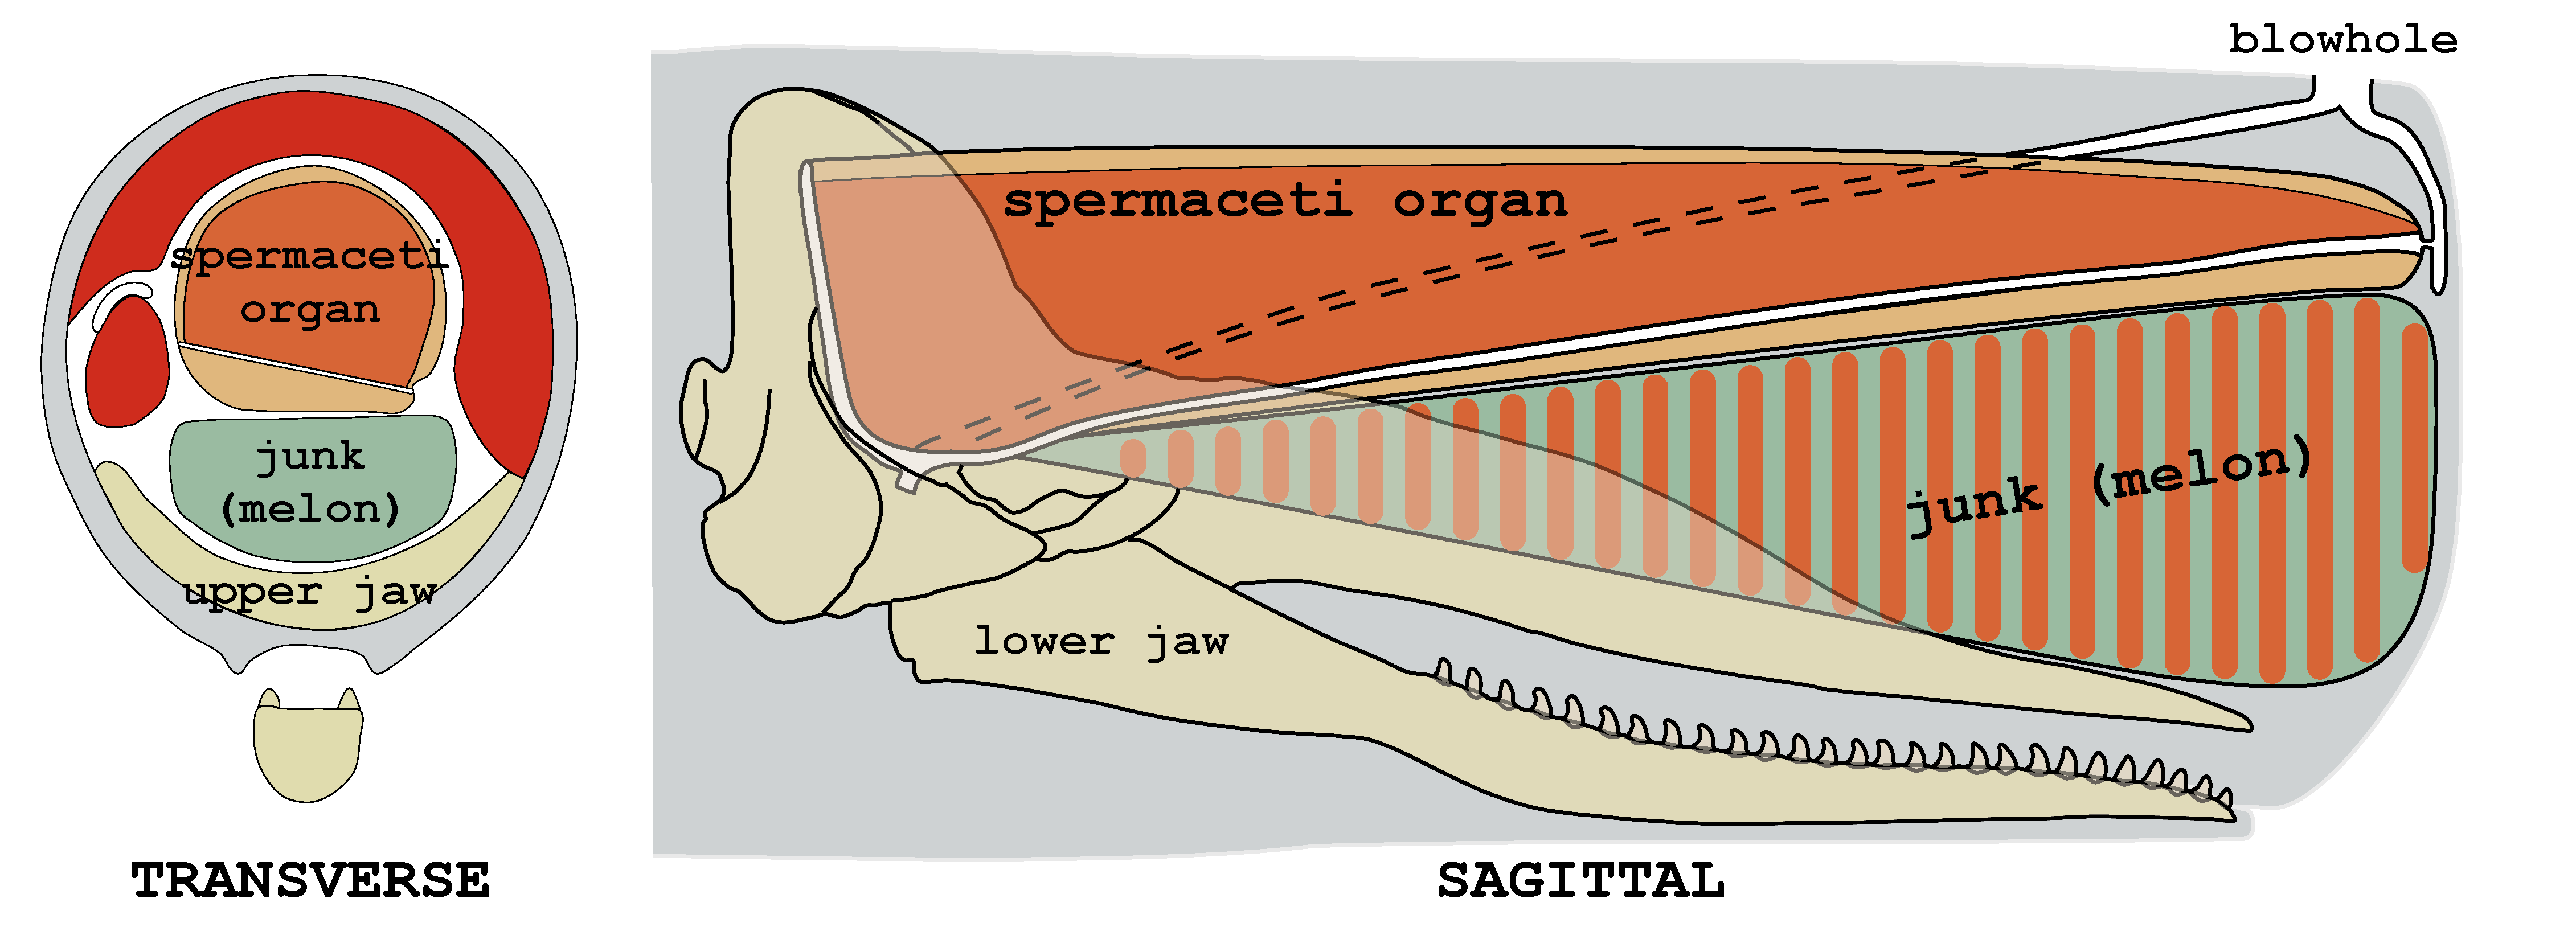
\includegraphics[width=0.9\textwidth]{figures/spermaceti.pdf}
        \caption[Spermaceti organ]{\footnotesize Outline of the spermaceti organ and the craneum architecture of the sperm whale. Both the spermaceti and the sponge-like melon are thought to participe in the complex resonance system described. Adapted from \textsl{WikiCommons}, Creative Commons license.}
        \label{f_spermaceti}
    \end{center}
\end{figure}

As a member of one of the few groups of mammals solely living in aqueous environments (Cetacea), sperm whales have undergone a process of adaptation to underwater distinctive features.
First and foremost, given the nature of water, gravity is much more forgiving with organisms, allowing them to reach larger sizes, which grant these creatures a series of attributes.
Thus, a link between longevity and size was already hinted by Aristotle in the \textsl{IV} century BC \cite{Speakman2005}. 
This link is particularly apparent in the case of Bowhead whales who, as we mentioned before, can live to up to 4 centuries.
In addition to that, as dictated by Peto's paradox, the observation of a moderate frequency of cancer occurrences in this gargantuan animals suggests extremely tight cancer protection mechanisms.
Namely, by virtue of having a very large body, cetaceans are made of a larger number of cells than other mammals, which means more cells potentially able to develop cancer-like mutations.
Therefore, this increase in cell number must be compensated by a much lower probability for tumorigenesis in each cell, accomplished via different systems \cite{Tollis2017a}.
Secondly, changes in pressure from shallow to deep waters demand different ways of regulation of blood homoeostasis (also known as \emph{haemostasis}) \cite{Stewart2009}.
This is especially important in the case of sperm whales, which, along with the Cuvier's whale, is one of the deepest divers known among mammals \cite{Schorr2014}.

On top of all of these features, sperm whales develop a distinctive skin structure, presenting a significant thicker \textsl{stratum corneum} than that of other Cetacea.
In addition to the tissue structure of the skin, it differs macroscopically from other cetaceans in which it is more wrinkled (sometimes it is compared to a raisin).
Also, sperm whales shed skin more regularly than other species \cite{Sokolov1982}.
Given the fact that skin is the first line of defence against the environment, these special traits may provide some advantage to the sperm whale in terms of physical defence, both against the attacks of their prey and the medium itself.
Thus, it has been proposed a relationship between the diving peculiarities of the sperm whale and those of its skin, maybe also weighting in its hunting habits \cite{Strauss1969}.

\subsection{Lonesome George and other giant tortoises} \label{ss_intro_models_giant_tortoises}

On September of 1835, \textsl{HMS Beagle} arrived to the shores of the Gal\'{a}pagos Archipelago to perform cartography mappings.
For some weeks, on-board naturalist and geologist Charles Darwin also observed and recollected data on the island biodiversity, which, eventually, along with other findings, helped him enact his theory of evolution by means of natural selection.
Among these observations, he noticed that the tortoises from different islands displayed conspicuous differences.
Even so, tortoises from the same island presented very diverse shells depending on the altitude of their habitat \cite{Darwin1845}.
Ever since, partly due its implication in the development of this theory, the Gal\'{a}pagos giant tortoises have become well known everywhere, and have greatly contributed to the well-deserved notoriety of the archipelago.
The most famous Gal\'{a}pagos tortoise was Lonesome George, the last member of his species, \textit{Chelonoidis abingdonii}, who tragically died in 2012, when believed to be ~101-102 years old, becoming an important symbol for conservation efforts, both in the Gal\'{a}pagos Islands and around the world.

At some point it was considered that all Gal\'{a}pagos tortoises were, in fact, one single species, \textit{Chelonoidis nigra}, composed of several subspecies (\textit{e.g.}, Lonesome George would have belonged to the subspecies \textit{C. nigra abingdonii}) \cite{Caccone1999}.
Nowadays, studies support the idea of several differentiated species, sharing the same genus (\textit{Chelonoidis}), but each independent \cite{Le2006}.

\begin{figure}[t!]
    \begin{center}
        \includegraphics[width=1\textwidth]{figures/galapagos.pdf}
        \caption[Gal\'{a}pagos giant tortoises and their habitat]{\footnotesize Representation of the Gal\'{a}pagos Island (names in \textbf{black}) and the Gal\'{a}pagos giant tortoises that inhabits them, indicating in \textcolor{myred1}{\textbf{red}} those that are currently extinct, in \textcolor{myora1}{\textbf{orange}} those in doubt, and in \textcolor{mygre2}{\textbf{green}} the rest. Adapted from \textsl{WikiCommons}, Creative Commons license.}
        \label{f_galapagos}
    \end{center}
\end{figure}

As a group, these species are all part of the class Reptilia (also referred to as Sauropsida).
Reptilia is a complex clade, since we must contemplate that birds are part of it in order to considerate it a monophyletic group, or to assume that it's paraphyletic (leaving crocodiles on a side).
The traditional approach went by considering 2 subdivision of this class, Diapsida, and Anapsida, which refers to the number of openings in their skulls (Diapsida having two of them, and Anapsida having none).
This classification,based on directly observable morphological features, has been revised and the current approach consist on 2 subdivisions as well, this time being Eureptilia, and Parareptilia \cite{Benton2014}.
While Parareptilia is extinct, Eureptilia contains itself another subdivision, called Diapsida, in which diapsides have being merged with anapsides, that has being rename as infraclass Neodiapsida.
Inside this infraclass, Testudinata constitutes an order on its own, while Lepidosauromorpha (Tuataras, lizards, and snakes) and Archosauromorpha (crocodiles and birds, along with dinosaurs), maintain their status of infraclasses (figure \ref{f_testudines_tree}) \cite{Mannen1999,Modesto2004}.

Turtles\footnote{Disclaimer: \quotes{Turtle} can refer to the order as a whole or, when differentiating between them, to the aquatic Testudines. In this sense, we use \quotes{tortoises} to refer to the land members of the order, while those able of both walking and swimming will be referred at as \quotes{terrapins}. Whenever talking about the specific varieties we will try to stick to the more specific names possible.} comprises more than 300 species \cite{Rhodin2017}.
This group is subdivided into two suborders, Pleurodira and Cryptodira, depending on whether their neck retracts sidewards or backwards, respectively.
The extant members of Pleurodira are largely restricted to fresh-water ecosystems \cite{Ferreira2018}. 
On the other hand, Cryptodira thrive in land, aquatic and mixed habitats.
They present different adaptations according to feeding, both herbivorous and carnivorous, not to mention sizes, ranging from some centimetres to more than 2 metres.
%Interestingly, many of the larger species have been reported to present a gigantism not linked to island gigantism\footnote{A phenomena by which an isolated specie tends to increase or reduce its size depending on his original inland size being small or big (respectively), by means of redistribution of tropic relations in the island ecosystem.}.

Another remarkable feature of turtles is their longevity.
Allegedly, one of the oldest turtles to ever live, \textsl{Adwaita} an Aldabra giant tortoise (\textit{A. gigantea}), reached more than 250 years.
Sadly no records are kept to support this claim.
Among those with recorded or tested age, \textsl{Tu'i Malila} (deceased in 1956) and \textsl{Jonathan} (still alive) are both 188 years old and are thus considered the longest lived terrestrial animals.
Notably, while \textsl{Jonathan} is also an Aldabra tortoise, \textsl{Tu'i Malila} was a member of \textit{Geochelone radiata}, one of the land relatives of Gal\'{a}pagos Giant tortoises (of a much smaller size).
Next in the list would be \textsl{Harriet}, a Gal\'{a}pagos giant tortoise (\textit{C. porteri}), who died in 2006 at the age of 176 years.
Another small tortoise, \textsl{Timothy}, lived 160 years, from around 1844 to 2004.
Timothy belonged to \textit{Testudo gracea}, also related to the land family of Gal\'{a}pagos giant tortoises.
In this sense, it has been discussed that the \quotes{early} dead of Lonesome George had some pathological component to it, but this doesn't make his age negligible.

%To cite other interesting characteristics in tortoises, it has been noted from an early time their capability to enter an \quotes{stasis} state, similar to hibernation, in which they can survive for almost a year without nutrients or water.
%For this reason they were used as a naturally preserved source of food in the long ship trips, including that of \textsl{H.M.S. Beagle}.
%Also, almost as a curiosity, in some zoological publications of the XIX century, a researcher reported movement and activity up to more than 15 days after surgically removing the head. 

\bigskip
\bigskip
\bigskip
All these long-lived metazoans must show genomic footprints of the evolutionary processes that lent them a combination of molecular characteristics that solve the problems associated with longevity.
With the intention of shedding some light on the subject of ageing, and to contribute to the collective efforts in solving this impending problem, the present Doctoral Thesis aims to study some of nature's solutions from an evolutionary point of view, paying special attention to the study of the degradome and its impact on longevity.

\vspace*{\fill}
